% !TEX root = Main.tex

\section{Theoretischer Hintergrund}
Um die nachfolgende Abschnitte verständlich zu machen ist eine kurze Erläuterung des theoretischen Hintergrunds sinnvoll.
\subsection{Verallgemeinerung}
Der zu entwickelnde Compiler nimmt als Eingabe eine Text-Datei mit Instruktionen in der Ausgangssprache. Der Compiler verarbeitet diese Eingabe und gibt als Ausgabe eine Datei mit Anweisungen in der Zielsprache zurück. Diese Verarbeitung kann grob in drei Abschnitte eingeteilt werden.
\subsubsection{Lexikalische Analyse}
Der erste Schritt ist dabei die sogenannte lexikalische Analyse. Die Eingabedatei ist für den Computer zunächst nur eine Kette von Zeichen. Diese Zeichen sind in sogenannte Tokens aufzuteilen. Beispielhaft könnte die Eingabe
\begin{lstlisting} [frame=single]
 a = b + c;
\end{lstlisting}

zu den folgenden Tokens aufgelöst werden.


\begin{figure}[h!]
\centering
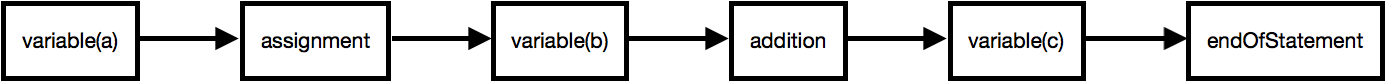
\includegraphics[scale=0.5]{pics/lex_beispiel.png}
\caption{Kurzes Beispiel für lexikalische Analyse}

\end{figure}

Der Teil des Compilers, der diese Aufgabe übernimmt, wird \textit{Lexer} genannt. Der Lexer überprüft für jedes Zeichen der Eingabedatei, welchem Token dieses zugeordnet werden kann. Dies geschieht auf Grundlage von definierten Regeln, welche mit sogenannten \textit{regulären Ausdrücken} formuliert werden. Ein regulärer Ausdruck besteht aus einer Sequenz von Zeichen, die ein bestimmtes Muster definieren. Reguläre Ausdrücke können auch rekursiv verwendet werden, um auf Grundlage einfacher regulärer Ausdrücke komplexere zu bilden. Beispiele für reguläre Ausdrücke werden im Kapitel \textit{\ref{subsec:arithExp}. Erste Schritte: Auswertung von arithmetischen Ausdrücken} aufgeführt.

\subsubsection{Syntaktische Analyse}
% TO-DO: Grafik
Im zweiten Schritt der Verarbeitung wird die \textit{syntaktische Analyse} durchgeführt. Dabei wird überprüft, ob die Eingabedatei einer definierten Grammatik entspricht, während bei der lexikalischen Analyse lediglich die übergebene Zeichenfolge in Tokens aufgeteilt wird, nicht jedoch überprüft wird, ob diese der Grammatik entsprechend zusammengeführt werden können. 

Bei einer erfolgreichen Auswertung wird die Folge an Tokens, die bei der lexikalischen Analyse ermittelt wurde, in einen Syntaxbaum übergeführt. Dies ist notwendig, um die Tokens in der richtigen Reihenfolge auszuwerten. 
%hier wäre eine Grafik auch hilfreich
%ich kümmere mich drum  -- lg marvin

\subsubsection{Syntaxgesteuerte Übersetzung}
Die eigentlich Erzeugung von Code in der Ausgangssprache findet zuletzt statt. Hierbei wird jeder Knoten des Syntaxbaum betrachtet und je nach Kontext eine Zeichenkette mit Anweisungen in der Zielsprache generiert. In diesem Schritt findet ebenfalls die semantische Analyse statt, beispielsweise die Überprüfung, ob eine aufgerufene Variable vorher deklariert wurde.
